\section{Protocol Decision Example}\label{sc:protocolDecisionExample}
Figure 10 (left) shows the base station RSSI of a run around the track from start to finish, while figure 10 (right) shows the base station RSSI for 47 rounds, which equals to a marathon, and each round has different fadings. Figure \ref{fig:recievedSignal_inRange_halfTrack} shows the in range of the base station packages which needs to be relayed or not.

%Figure 10
%TODO Find matlab document med de to figures i word

%Figure 11
\begin{figure}[H]
	\centering
	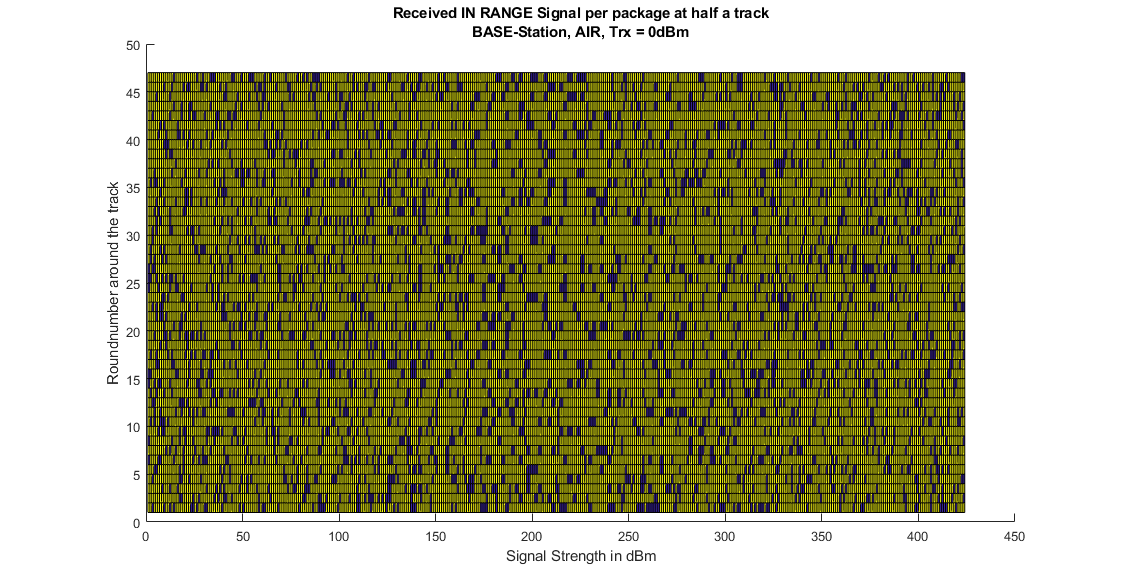
\includegraphics[width=\linewidth]{theory/protocolDecisionExample/fig/recievedSignal_inRange_halfTrack.png}
	\caption{In, half a track, base station RSSI transmitting range ToHopOrNot plot. Blue is relayed packages while yellow is direct package.}
	\label{fig:recievedSignal_inRange_halfTrack}
\end{figure}

A multi-linear regression line estimation was process on the simulated data based on distance, signal strength and package status, relayed or not, trying to determine whether to relay or not the next package. Since in our simulation signal strength and distance are strongly correlated, due to antenna approximation and the binary behaviour of the fading, they cancel each other out, while the previous package status shows a $10\%$ likelihood of the next package needing to be relayed. Again, it is also expected since the simulations have fading behaviour added as a random variable appearing randomly at a $10\%$ likelihood. A real-life excursion of the case would be interesting to see the analysis on, but it, unfortunately, is a bit out of scope for the project. Figure \ref{fig:regressionPlot} show the regression plot with the equation added as a legend box.

%Figure 12
\begin{figure}[H]
	\centering
	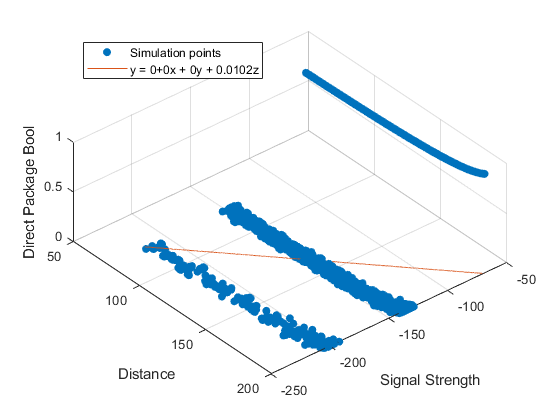
\includegraphics[width=\linewidth]{theory/protocolDecisionExample/fig/regressionPlot.png}
	\caption{Regression plot of the three variables, distance, RSSI and Relayed or not packages. The regression line is representing a change from direct transmission to relaying.}
	\label{fig:regressionPlot}
\end{figure}